% Created by tikzDevice version 0.12.6 on 2025-11-05 12:08:39
% !TEX encoding = UTF-8 Unicode
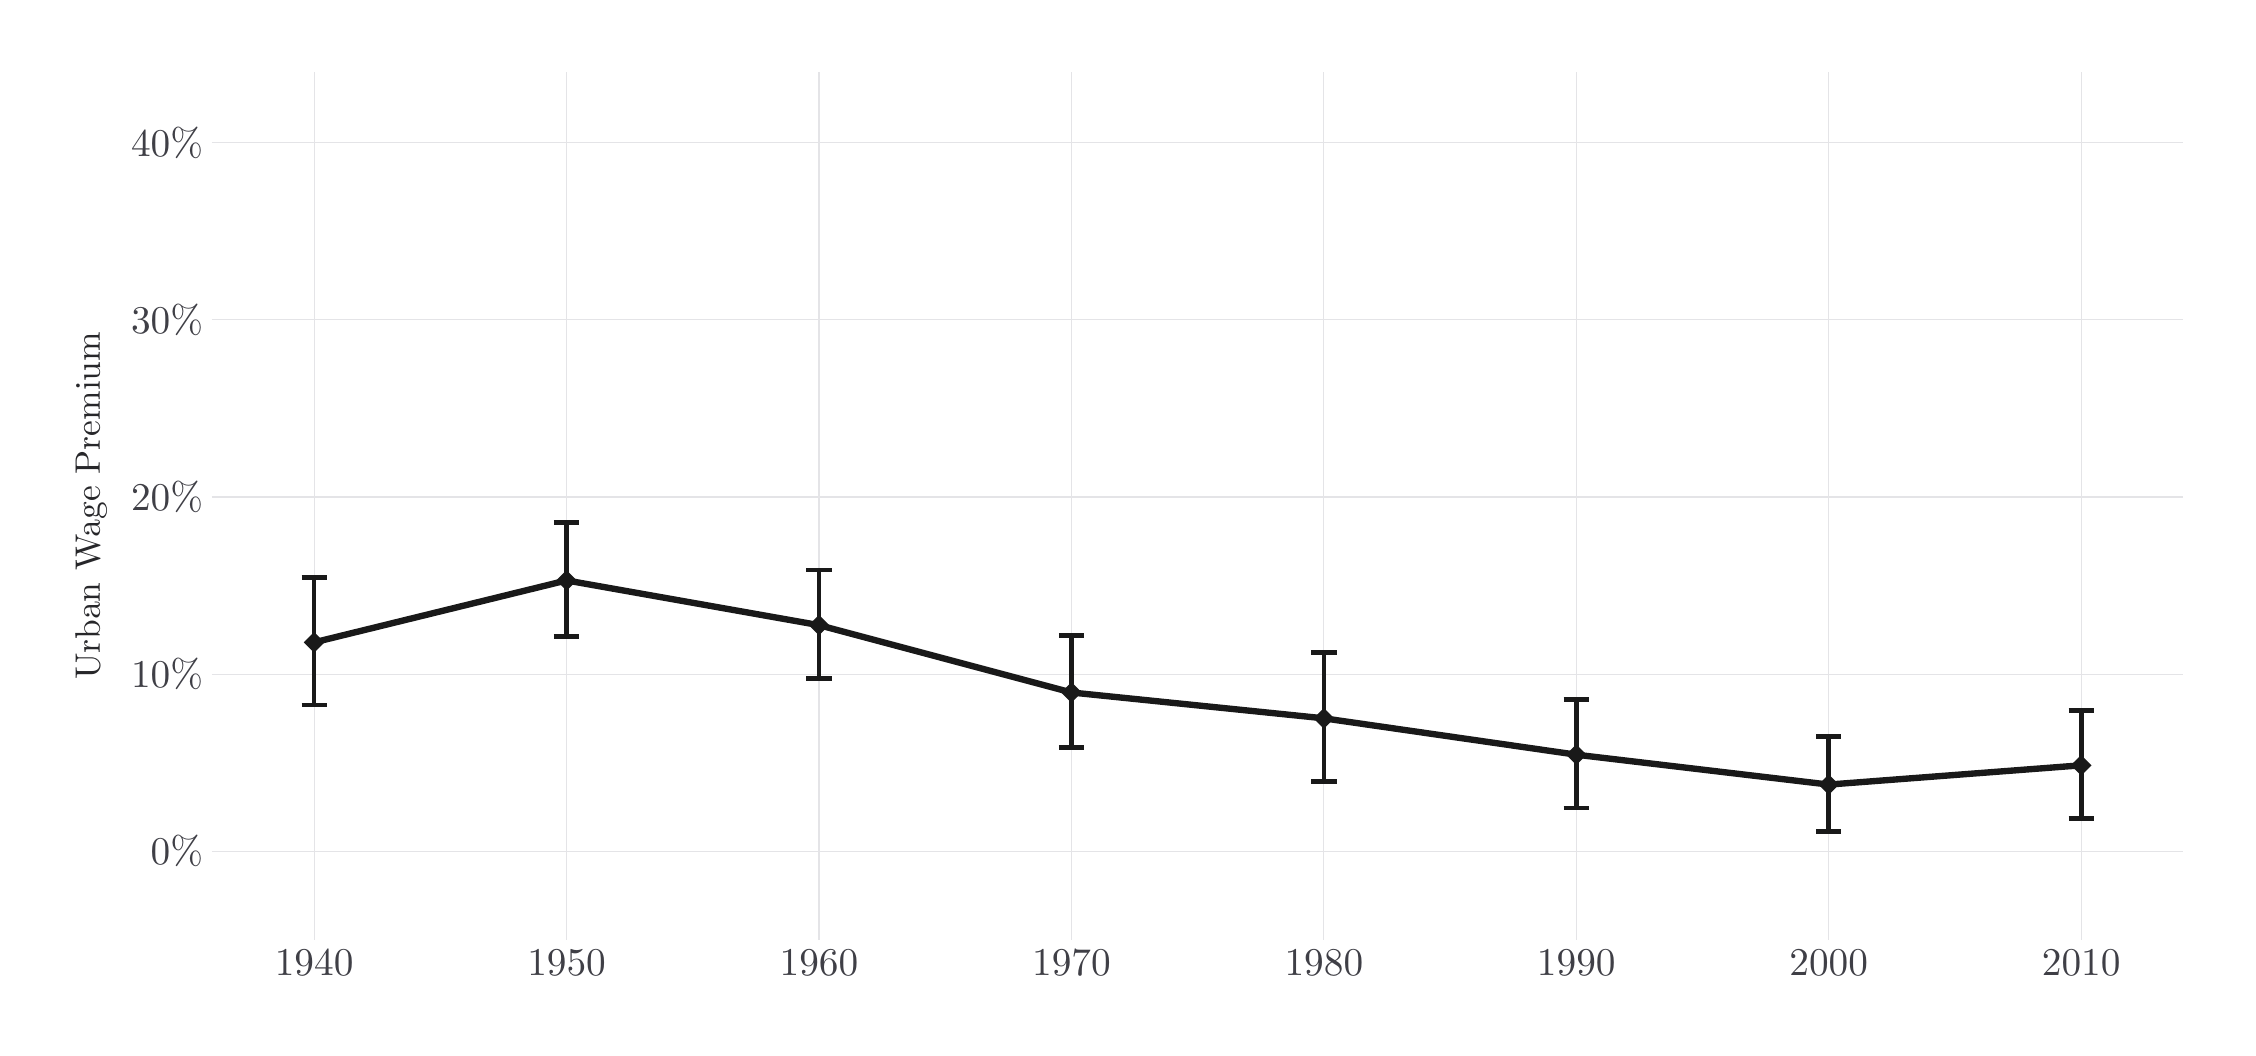
\begin{tikzpicture}[x=1pt,y=1pt]
\definecolor{fillColor}{RGB}{255,255,255}
\path[use as bounding box,fill=fillColor] (0,0) rectangle (794.97,361.35);
\begin{scope}
\path[clip] (  0.00,  0.00) rectangle (794.97,361.35);
\definecolor{drawColor}{RGB}{255,255,255}

\path[draw=drawColor,line width= 0.8pt,line join=round,line cap=round,fill=fillColor] (  0.00,  0.00) rectangle (794.97,361.35);
\end{scope}
\begin{scope}
\path[clip] ( 66.57, 31.76) rectangle (778.97,345.35);
\definecolor{drawColor}{RGB}{255,255,255}
\definecolor{fillColor}{RGB}{255,255,255}

\path[draw=drawColor,line width= 0.8pt,line join=round,line cap=round,fill=fillColor] ( 66.57, 31.76) rectangle (778.97,345.35);
\definecolor{drawColor}{RGB}{228,228,231}

\path[draw=drawColor,line width= 0.4pt,line join=round] ( 66.57, 63.76) --
	(778.97, 63.76);

\path[draw=drawColor,line width= 0.4pt,line join=round] ( 66.57,127.76) --
	(778.97,127.76);

\path[draw=drawColor,line width= 0.4pt,line join=round] ( 66.57,191.75) --
	(778.97,191.75);

\path[draw=drawColor,line width= 0.4pt,line join=round] ( 66.57,255.75) --
	(778.97,255.75);

\path[draw=drawColor,line width= 0.4pt,line join=round] ( 66.57,319.75) --
	(778.97,319.75);

\path[draw=drawColor,line width= 0.4pt,line join=round] (103.51, 31.76) --
	(103.51,345.35);

\path[draw=drawColor,line width= 0.4pt,line join=round] (194.73, 31.76) --
	(194.73,345.35);

\path[draw=drawColor,line width= 0.4pt,line join=round] (285.94, 31.76) --
	(285.94,345.35);

\path[draw=drawColor,line width= 0.4pt,line join=round] (377.16, 31.76) --
	(377.16,345.35);

\path[draw=drawColor,line width= 0.4pt,line join=round] (468.38, 31.76) --
	(468.38,345.35);

\path[draw=drawColor,line width= 0.4pt,line join=round] (559.59, 31.76) --
	(559.59,345.35);

\path[draw=drawColor,line width= 0.4pt,line join=round] (650.81, 31.76) --
	(650.81,345.35);

\path[draw=drawColor,line width= 0.4pt,line join=round] (742.03, 31.76) --
	(742.03,345.35);
\definecolor{drawColor}{gray}{0.10}

\path[draw=drawColor,line width= 2.3pt,line join=round] (103.51,139.23) --
	(194.73,161.61) --
	(285.94,145.45) --
	(377.16,121.12) --
	(468.38,111.78) --
	(559.59, 98.64) --
	(650.81, 87.84) --
	(742.03, 94.80);

\path[draw=drawColor,line width= 1.7pt,line join=round] ( 98.95,162.60) --
	(108.07,162.60);

\path[draw=drawColor,line width= 1.7pt,line join=round] (103.51,162.60) --
	(103.51,116.59);

\path[draw=drawColor,line width= 1.7pt,line join=round] ( 98.95,116.59) --
	(108.07,116.59);

\path[draw=drawColor,line width= 1.7pt,line join=round] (190.17,182.48) --
	(199.29,182.48);

\path[draw=drawColor,line width= 1.7pt,line join=round] (194.73,182.48) --
	(194.73,141.32);

\path[draw=drawColor,line width= 1.7pt,line join=round] (190.17,141.32) --
	(199.29,141.32);

\path[draw=drawColor,line width= 1.7pt,line join=round] (281.38,165.34) --
	(290.50,165.34);

\path[draw=drawColor,line width= 1.7pt,line join=round] (285.94,165.34) --
	(285.94,126.09);

\path[draw=drawColor,line width= 1.7pt,line join=round] (281.38,126.09) --
	(290.50,126.09);

\path[draw=drawColor,line width= 1.7pt,line join=round] (372.60,141.68) --
	(381.72,141.68);

\path[draw=drawColor,line width= 1.7pt,line join=round] (377.16,141.68) --
	(377.16,101.15);

\path[draw=drawColor,line width= 1.7pt,line join=round] (372.60,101.15) --
	(381.72,101.15);

\path[draw=drawColor,line width= 1.7pt,line join=round] (463.82,135.47) --
	(472.94,135.47);

\path[draw=drawColor,line width= 1.7pt,line join=round] (468.38,135.47) --
	(468.38, 88.88);

\path[draw=drawColor,line width= 1.7pt,line join=round] (463.82, 88.88) --
	(472.94, 88.88);

\path[draw=drawColor,line width= 1.7pt,line join=round] (555.03,118.47) --
	(564.15,118.47);

\path[draw=drawColor,line width= 1.7pt,line join=round] (559.59,118.47) --
	(559.59, 79.38);

\path[draw=drawColor,line width= 1.7pt,line join=round] (555.03, 79.38) --
	(564.15, 79.38);

\path[draw=drawColor,line width= 1.7pt,line join=round] (646.25,105.28) --
	(655.37,105.28);

\path[draw=drawColor,line width= 1.7pt,line join=round] (650.81,105.28) --
	(650.81, 70.85);

\path[draw=drawColor,line width= 1.7pt,line join=round] (646.25, 70.85) --
	(655.37, 70.85);

\path[draw=drawColor,line width= 1.7pt,line join=round] (737.47,114.57) --
	(746.59,114.57);

\path[draw=drawColor,line width= 1.7pt,line join=round] (742.03,114.57) --
	(742.03, 75.61);

\path[draw=drawColor,line width= 1.7pt,line join=round] (737.47, 75.61) --
	(746.59, 75.61);
\definecolor{fillColor}{gray}{0.10}

\path[fill=fillColor] ( 99.78,139.23) --
	(103.51,142.96) --
	(107.24,139.23) --
	(103.51,135.50) --
	cycle;

\path[fill=fillColor] (191.00,161.61) --
	(194.73,165.34) --
	(198.46,161.61) --
	(194.73,157.88) --
	cycle;

\path[fill=fillColor] (282.21,145.45) --
	(285.94,149.18) --
	(289.67,145.45) --
	(285.94,141.72) --
	cycle;

\path[fill=fillColor] (373.43,121.12) --
	(377.16,124.85) --
	(380.89,121.12) --
	(377.16,117.39) --
	cycle;

\path[fill=fillColor] (464.65,111.78) --
	(468.38,115.51) --
	(472.11,111.78) --
	(468.38,108.05) --
	cycle;

\path[fill=fillColor] (555.86, 98.64) --
	(559.59,102.37) --
	(563.32, 98.64) --
	(559.59, 94.91) --
	cycle;

\path[fill=fillColor] (647.08, 87.84) --
	(650.81, 91.57) --
	(654.54, 87.84) --
	(650.81, 84.11) --
	cycle;

\path[fill=fillColor] (738.30, 94.80) --
	(742.03, 98.53) --
	(745.76, 94.80) --
	(742.03, 91.07) --
	cycle;
\end{scope}
\begin{scope}
\path[clip] (  0.00,  0.00) rectangle (794.97,361.35);
\definecolor{drawColor}{RGB}{63,63,70}

\node[text=drawColor,anchor=base east,inner sep=0pt, outer sep=0pt, scale=  1.42] at ( 63.37, 58.86) {0\%};

\node[text=drawColor,anchor=base east,inner sep=0pt, outer sep=0pt, scale=  1.42] at ( 63.37,122.86) {10\%};

\node[text=drawColor,anchor=base east,inner sep=0pt, outer sep=0pt, scale=  1.42] at ( 63.37,186.86) {20\%};

\node[text=drawColor,anchor=base east,inner sep=0pt, outer sep=0pt, scale=  1.42] at ( 63.37,250.86) {30\%};

\node[text=drawColor,anchor=base east,inner sep=0pt, outer sep=0pt, scale=  1.42] at ( 63.37,314.85) {40\%};
\end{scope}
\begin{scope}
\path[clip] (  0.00,  0.00) rectangle (794.97,361.35);
\definecolor{drawColor}{RGB}{63,63,70}

\node[text=drawColor,anchor=base,inner sep=0pt, outer sep=0pt, scale=  1.42] at (103.51, 18.76) {1940};

\node[text=drawColor,anchor=base,inner sep=0pt, outer sep=0pt, scale=  1.42] at (194.73, 18.76) {1950};

\node[text=drawColor,anchor=base,inner sep=0pt, outer sep=0pt, scale=  1.42] at (285.94, 18.76) {1960};

\node[text=drawColor,anchor=base,inner sep=0pt, outer sep=0pt, scale=  1.42] at (377.16, 18.76) {1970};

\node[text=drawColor,anchor=base,inner sep=0pt, outer sep=0pt, scale=  1.42] at (468.38, 18.76) {1980};

\node[text=drawColor,anchor=base,inner sep=0pt, outer sep=0pt, scale=  1.42] at (559.59, 18.76) {1990};

\node[text=drawColor,anchor=base,inner sep=0pt, outer sep=0pt, scale=  1.42] at (650.81, 18.76) {2000};

\node[text=drawColor,anchor=base,inner sep=0pt, outer sep=0pt, scale=  1.42] at (742.03, 18.76) {2010};
\end{scope}
\begin{scope}
\path[clip] (  0.00,  0.00) rectangle (794.97,361.35);
\definecolor{drawColor}{RGB}{39,39,42}

\node[text=drawColor,rotate= 90.00,anchor=base,inner sep=0pt, outer sep=0pt, scale=  1.28] at ( 26.06,188.55) {Urban Wage Premium};
\end{scope}
\end{tikzpicture}
